%%%%%%%%%%%%%%%%%%%%%%%%%%%%%%%%%%%%%%%%%%%%%%%%%%%%%%%
%% Engineer & Master Thesis, LaTeX Template          %%
%% Copyleft by Piotr Woźniak & Artur M. Brodzki      %%
%% Faculty of Electronics and Information Technology %%
%% Warsaw University of Technology, Warsaw, 2019     %%
%%%%%%%%%%%%%%%%%%%%%%%%%%%%%%%%%%%%%%%%%%%%%%%%%%%%%%%

\documentclass[
    left=2.0cm,         % Sadly, generic margin parameter
    right=2.0cm,        % doesnt't work, as it is
    top=2.0cm,          % superseded by more specific
    bottom=2.5cm,         % left...bottom parameters.
    bindingoffset=6mm,  % Optional binding offset.
    nohyphenation=false % You may turn off hyphenation, if don't like. 
]{eiti/eiti-thesis}

\usepackage[spanish]{babel}
\usepackage[
    backend=bibtex,
    style=ieee
]{biblatex}
\usepackage{csquotes}
\usepackage{multirow}
\usepackage[table,xcdraw]{xcolor}

\graphicspath{{img/}}             % Katalog z obrazkami.
\addbibresource{bibliografia.bib} % Plik .bib z bibliografią




%----------------------------------------
% Twierdzenia i definicje;
% tutaj ew. tłumaczymy te terminy
% na inne języki
%----------------------------------------
\newtheorem{theorem}{Teorema}
\newtheorem{lemma}{Lema}
\newtheorem{corollary}{Corolario}
\newtheorem{definition}{Definicion}
\newtheorem{axiom}{Axioma}
\newtheorem{assumption}{Supuesto}

%----------------------------------------
% Spis rysunków, tablic i załączników;
% tutaj ew. tłumaczymy te terminy
% na inne języki
%----------------------------------------
\AtBeginDocument{
    \renewcommand{\listfigurename}{Figura}
    \renewcommand{\listtablename}{Tabla}
    \renewcommand{\tablename}{Tabela}
}

\begin{document}

%--------------------------------------
% Strona tytułowa
%--------------------------------------
\EngineerThesis % dla pracy inżynierskiej mamy \EngineerThesis
\instytut{XXXXXX}
\kierunek{XXXXXX}
\specjalnosc{XXXXXX}
\title{
    Predicción de sitios de unión en proteínas \\
    usando redes neuronales de grafos
}
\author{\{Joaquin Torre Zaffaroni\}}
\album{XXXXXX}
\promotor{XXXXXX}
\date{\the\year}
\maketitle

%--------------------------------------
% Streszczenie po polsku
%--------------------------------------
%\resumen Podar lo de abajo
%\palabrasclave virtual screening, graph neural networks
%\newpage

%--------------------------------------
% Streszczenie po angielsku
%--------------------------------------
%\abstract \kant[1-3]
%\keywords XXX, XXX, XXX
%\newpage

%--------------------------------------
% Oświadczenie o autorstwie
%--------------------------------------
%\makeauthorship
%\blankpage

%--------------------------------------
% Spis treści
%--------------------------------------
%\thispagestyle{empty}
\tableofcontents
\newpage
%\cleardoublepage

%--------------------------------------
% Rozdziały
%--------------------------------------
%\newpage % Zaleca się otwieranie rozdziału od nowej strony.
\section[Wstęp]{Wstęp}
\lipsum[1] \cite{goossens93}
\begin{figure}[!h]
    \label{fig:anzelm}
    \centering 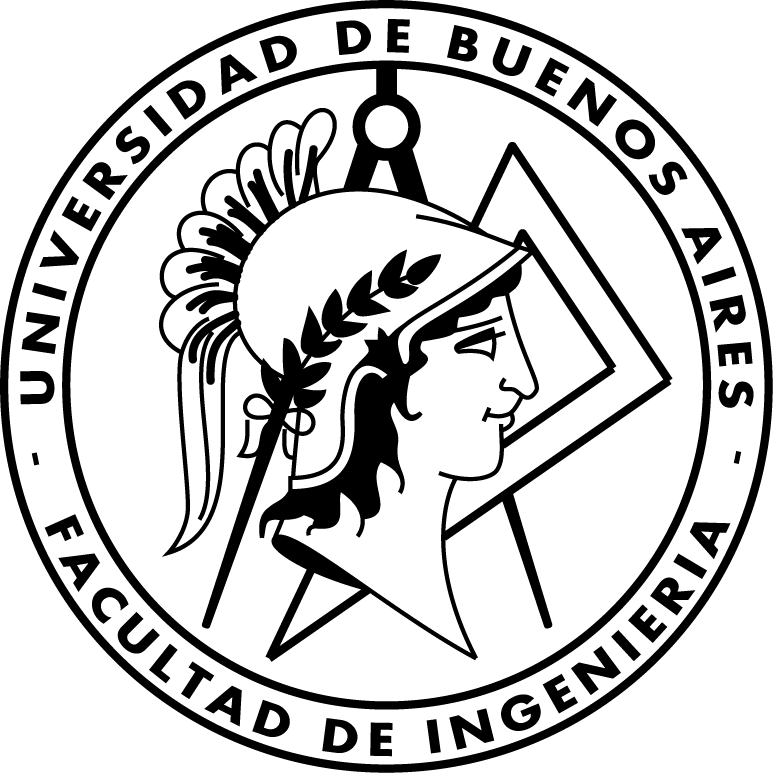
\includegraphics[width=0.5\linewidth]{logo_fiuba.png}
    \caption{CaptionLogo.}
\end{figure}
\lipsum[2-10]
         % W długich pracach
%\newpage % Zaleca się otwieranie rozdziału od nowej strony.
\section{De Finibus Bonorum et Malorum}
\lipsum[1] Lorem ipsum dolor sit amet\footnote{Lorem ipsum dolor sit amet, consectetur adipiscing elit, sed do eiusmod tempor incididunt ut labore et dolore magna aliqua. Ut enim ad minim veniam, quis nostrud exercitation ullamco laboris nisi ut aliquip ex ea commodo consequat.}. 
\begin{align*}
    E & = mc^2 \\ 
    y & = ax^2 + bx + c
\end{align*}

\lipsum[3]

\begin{align}
\begin{bmatrix}
    1 & 0 & 0 \\ 
    0 & 2 & 0 \\ 
    0 & 0 & 3
\end{bmatrix} \cdot 
\begin{bmatrix}
    4 \\ 5 \\ 6
\end{bmatrix} = 
\begin{bmatrix}
    4 \\ 10 \\ 18
\end{bmatrix}
\end{align}

\lipsum[4] Lorem ipsum dolor sit amet, consectetur adipiscing elit, sed do eiusmod tempor incididunt ut labore et dolore magna aliqua \cite{szczypiorski2015}, \cite{duqu2011}, \cite{shs2015}, \cite{wozniak2018}, \cite{dcp19}. 

\subsection{Critique of Pure Reason}
\kant[1]

\begin{table}[!h] \label{tab:tabela1} \centering
\caption{Przykładowa tabela.}
\begin{tabular} {| c | c | r |} \hline
    Kolumna 1 & Kolumna 2 & Liczba \\ \hline\hline
    cell1 & cell2 & 60 \\ \hline
    cell4 & cell5 & 43 \\ \hline
    cell7 & cell8 & 20,45 \\ \hline
    \multicolumn{2}{|r|}{Suma:} & 123,45 \\ \hline
\end{tabular}
\end{table}

\kant[2]

\begin{longtable}{| c | m{0.58\linewidth} | r | m{0.1\linewidth} |} 
    \caption{Tabela wielostronicowa.} \\ 
    \hline
    Lp & \multicolumn{1}{c|}{Treść} & \multicolumn{1}{c|}{Kwota} & \multicolumn{1}{m{0.1\linewidth}|}{Wariant opłaty} \\ \hline\hline \endfirsthead
    
    \endfoot
    \hline \endlastfoot
    
    1 & Lorem ipsum dolor sit amet, consectetur adipiscing elit, sed do eiusmod tempor incididunt ut labore et dolore magna aliqua. & 111 111,11 zł & \multicolumn{1}{c|}{WAR1} \\ \hline
    2 & Lorem ipsum dolor sit amet, consectetur adipiscing elit, sed do eiusmod tempor incididunt ut labore et dolore magna aliqua. & 22 222,22 zł & \multicolumn{1}{c|}{WAR1} \\ \hline
    3 & Lorem ipsum dolor sit amet, consectetur adipiscing elit, sed do eiusmod tempor incididunt ut labore et dolore magna aliqua. & 33 333,33 zł & \multicolumn{1}{c|}{WAR1} \\ \hline
    4 & Lorem ipsum dolor sit amet, consectetur adipiscing elit, sed do eiusmod tempor incididunt ut labore et dolore magna aliqua. & 444 444,44 zł & \multicolumn{1}{c|}{WAR1} \\ \hline
    5 & Lorem ipsum dolor sit amet, consectetur adipiscing elit, sed do eiusmod tempor incididunt ut labore et dolore magna aliqua. & 55 555,55 zł & \multicolumn{1}{c|}{WAR1} \\ \hline
    6 & Lorem ipsum dolor sit amet, consectetur adipiscing elit, sed do eiusmod tempor incididunt ut labore et dolore magna aliqua. & 66 666,66 zł & \multicolumn{1}{c|}{WAR1} \\ \hline
    7 & Lorem ipsum dolor sit amet, consectetur adipiscing elit, sed do eiusmod tempor incididunt ut labore et dolore magna aliqua. & 777 777,77 zł & \multicolumn{1}{c|}{WAR1} \\ \hline
    8 & Lorem ipsum dolor sit amet, consectetur adipiscing elit, sed do eiusmod tempor incididunt ut labore et dolore magna aliqua. & 8 888,88 zł & \multicolumn{1}{c|}{WAR1} \\ \hline
    9 & Lorem ipsum dolor sit amet, consectetur adipiscing elit, sed do eiusmod tempor incididunt ut labore et dolore magna aliqua. & 999 999,99 zł & \multicolumn{1}{c|}{WAR1} \\ \hline
    10 & Lorem ipsum dolor sit amet, consectetur adipiscing elit, sed do eiusmod tempor incididunt ut labore et dolore magna aliqua. & 111 111,11 zł & \multicolumn{1}{c|}{WAR2} \\ \hline
    11 & Lorem ipsum dolor sit amet, consectetur adipiscing elit, sed do eiusmod tempor incididunt ut labore et dolore magna aliqua. & 22 222,22 zł & \multicolumn{1}{c|}{WAR2} \\ \hline
    12 & Lorem ipsum dolor sit amet, consectetur adipiscing elit, sed do eiusmod tempor incididunt ut labore et dolore magna aliqua. & 33 333,33 zł & \multicolumn{1}{c|}{WAR2} \\ \hline
    13 & Lorem ipsum dolor sit amet, consectetur adipiscing elit, sed do eiusmod tempor incididunt ut labore et dolore magna aliqua. & 444 444,44 zł & \multicolumn{1}{c|}{WAR2} \\ \hline
    14 & Lorem ipsum dolor sit amet, consectetur adipiscing elit, sed do eiusmod tempor incididunt ut labore et dolore magna aliqua. & 55 555,55 zł & \multicolumn{1}{c|}{WAR2} \\ \hline
    15 & Lorem ipsum dolor sit amet, consectetur adipiscing elit, sed do eiusmod tempor incididunt ut labore et dolore magna aliqua. & 66 666,66 zł & \multicolumn{1}{c|}{WAR2} \\ \hline
    & \multicolumn{1}{r|}{\textbf{Suma:}} & \textbf{7 777 777,77 zł} & 
    \label{table:koszty}
\end{longtable}
\kant[4]

\subsection{Categorical Imperative}
As any dedicated reader can clearly see, the Ideal of practical reason is a representation of, as far as I know, the things in themselves; as I have shown elsewhere, the phenomena should only be used as a canon for our understanding:
% Parametr label ustawia symbol, a leftmargin - wielkość wcięcia.
% Domyślny układ to [---] bez wcięcia, bo tak pan Marcin Woliński powiedział;
% ale ja nie polecam. // AB
\begin{itemize}
    \item Item 1:
    \begin{itemize}[label=---]
        \item item 1.1;
        \item item 1.2;
        \item item 1.3;
    \end{itemize}
    \item Item 2;
    \item Item 3;
    \item Item 4.
\end{itemize}
\kant[2]
\begin{enumerate}
    \item Item 1:
    \begin{enumerate}
        \item item 1.1;
        \item item 1.2:
        \begin{enumerate}
            \item item 1.2.1;
            \item item 1.2.2;
        \end{enumerate}
        \item item 1.3;
    \end{enumerate}
    \item Item 2;
    \item Item 3;
    \item Item 4.
\end{enumerate}

\kant[9]

\subsection{G\"odel's ontological proof}
\kant[9] Lorem ipsum dolor sit amet, consectetur adipiscing elit, sed do eiusmod tempor incididunt ut labore et dolore magna aliqua \cite{benzmuller2014}, \cite{goedel95}, \cite{wang97}, \cite{koons2005}. 
\begin{assumption} \label{ass:1}
    $ [\![ \ \phi \ ]\!] \Longrightarrow [\![ \ P(\phi); \neg P(\phi) \ ]\!]$
\end{assumption}
\begin{axiom}[Dualność] \label{axiom:1}
    $\neg P(\phi) \Leftrightarrow P(\neg \phi)$, równoważnie $P(\phi) \Leftrightarrow \neg P(\neg \phi)$
\end{axiom}
\begin{axiom}[Całkowitość] \label{axiom:2}
    $ \left( P(\phi) \wedge \forall x: \phi(x) \Rightarrow \psi(x) \right) \Rightarrow P(\psi) $
\end{axiom}
\begin{axiom}[Absolutność] \label{axiom:3}
    $ P(\phi) \Rightarrow \Box P(\phi) $
\end{axiom}
\begin{definition} \label{def:1}
    $ G(x) \Leftrightarrow \forall \phi: \left( P(\phi) \Rightarrow \phi(x) \right) $
\end{definition}
\begin{definition} \label{def:2}
    $ \phi \ ess \ x \Leftrightarrow \phi(x) \wedge \forall \psi \left( \psi(x) \Rightarrow \Box \forall y \left( \phi(y) \Rightarrow \psi(y) \right) \right)  $
\end{definition}
\begin{axiom} \label{axiom:4}
    P(G)
\end{axiom}
\begin{lemma} \label{lemma:1}
    $ P(\phi) \Rightarrow \Diamond \exists x : \phi(x) $
\end{lemma}
\begin{proof}
    Dowód pomijamy, bo jest trywialny :)
\end{proof}
\begin{lemma} \label{lemma:2}
    $ \Diamond \exists x : G(x) $
\end{lemma}
\begin{proof}
    Natychmiastowy wniosek z aksjomatu \ref{axiom:4} i lematu \ref{lemma:1}.
\end{proof}
\begin{lemma} \label{lemma:3}
    $ G(x) \Rightarrow G \ ess \ x $
\end{lemma}
\begin{proof}
    Poprzez podstawienie do definicji \ref{def:2}. 
\end{proof}
\begin{definition} \label{def:3}
    $ E(x) \Leftrightarrow \forall \phi \left( \phi \ ess \ x \Rightarrow \Box\ \exists x: \phi(x) \right) $
\end{definition}
\begin{axiom} \label{axiom:5}
    P(E)
\end{axiom}
\begin{theorem}
    $ \Box\ \exists x : G(x) $
\end{theorem}
\begin{proof}
    Na podstawie definicji \ref{def:1}, lematu \ref{lemma:3} i aksjomatu \ref{axiom:5}. 
\end{proof}    % wygodnie jest trzymać
%\newpage % Zaleca się otwieranie rozdziału od nowej strony.
\section{Code listings}
\lipsum[10]
\begin{lstlisting}[language=HTML]
<html>
  <head>
    <title>Hello world!</title>
  </head>
  <body>
    Hello
  </body>
</html>
\end{lstlisting}
\lipsum[11]
\begin{lstlisting}[language=C]
#include <stdio.h>
int main() {
  // printf() displays the string inside quotation
  printf("Hello world!");
  return 0;
}
\end{lstlisting}
\lipsum[12]
 % każdy rozdział w osobnym pliku. 

%\newpage % Zaleca się otwieranie rozdziału od nowej strony
\section{Introducción}

%discovering Side effects. diseño de drogas (leskovec en ML?)


Paul Ehrlich, premio Nobel de Medicina y luego inventor del primer tratamiento 
efectivo contra la sífilis, popularizó en el 1900 el concepto de la \textit{bala mágica}.
La idea marca que podría ser posible matar ciertos microbios causantes de enfermedades
sin lastimar al cuerpo. Un agente que cumpla esto actuaría como una bala que mágicamente
ataca a ciertos objetivos específicos, dejando intactos a otros. El primer fármaco
considerado como tal fue la arsfenamina, descubierta por Ehrlich para el uso del
tratamiento contra la sífilis. 

Como es conocido, el descubrimiento de la penicilina fue por accidente. El proceso
de sistematizar el entendimiento de qué compuestos podrían servir para tratar ciertas 
enfermedades se llama \textit{descubrimiento de drogas}. El enfoque más común en
la actualidad es el de \textit{farmacología inversa}: se identifican 
proteínas que están asociadas al comportamiento de la patología, 
se buscan compuestos que modulen
(reduzcan) su actividad y luego se hacen pruebas \textit{in vivo}. El proceso de
probar si una molécula pequeña puede modular la actividad de una proteína se
conoce como \textit{screening} (cribaje), y a esas proteínas se las conoce como
\textit{blancos terapéuticos}.

Una forma automatizada de hacer esto es por medio de \textit{virtual screening}.
Esta técnica permite predecir la capacidad de unión entre una droga y el 
receptor de una proteína.
En este trabajo nos enfocamos en un problema particular de esta técnica,
que es la evaluación de los lugares de la proteína donde se puede
unir un ligando particular (\textit{binding site prediction}). Por ejemplo,
no estamos determinando qué orientación tendrá el compuesto en la cavidad
(que se resuelve con técnicas de \textit{docking}), ni la afinidad
particular de una proteína contra distintas drogas. Puntualmente,
utilizaremos métodos de aprendizaje automático para resolver este problema.

%rever si este párrafo va acá o en otra sección

Para utilizar cualquier método de \textit{machine learning} es necesario
tener una manera de representar a los datos. Las proteínas, en principio,
se pueden modelar como secuencias de aminoácidos. Conociendo la secuencia
es posible determinar la estructura secundaria (plegamientos tridimensionales
entre aminoácidos cercanos) y la estructura terciaria (las posiciones
tridimensionales de todos los átomos); dado esto, es natural pensar que
la mejor forma de representar a la proteína es con su secuencia.
Sin embargo, el mapeo automático de la secuencia a la
estructura no es trivial. Como el problema de sitios de unión es un
fenómeno en el espacio, es mejor representar la estructura terciaria 
(las posiciones) y no la estructura primaria (la secuencia).
Como datos usaremos estructuras conseguidas experimentalmente, a través de
técnicas como la cristalografía de rayos X, que están disponibles en el 
\textit{Protein Data Bank}\footnote{http//wwpdb.org}, aunque también puede 
haber \textit{features} de otras fuentes.

\section{Contexto y estado del arte}
\subsection{Redes neuronales de grafos}

En general, una red neuronal es un modelo predictivo que tiene una capa de entrada, %curso de stanford
una capa de salida y una o varias capas intermedias que se denominan \textbf{capas
ocultas}. Por ejemplo, un perceptrón multicapa tiene capas con la siguiente forma:

\begingroup
 $$\mathbf{h}^{n+1} = \bar{\sigma}(\mathbf{W h}^{n} + \mathbf{b})$$
\endgroup


donde $h^n$ es la capa enésima de dimensión $N$, $h^{n+1}$ es la capa siguiente de
dimensión $M$, $W$ es una matriz de dimensión $M\times N$, $b$ es un vector de
sesgo y $\bar\sigma$ es la función de activación. Lo fundamental es que las
capas siguientes se relacionan con las anteriores según una función diferenciable
(para poder entrenar al modelo con \textit{backpropagation}). Por lo general la
capa final es \textit{softmax} \cite{sfunsupervised}, que es un predictor 
multiclase basado en hiperplanos. Como tal, las capas anteriores 
resuelven el problema de representación \cite{nielsen2015neural}.

Por eso, en redes neuronales que trabajan con imágenes se utilizan capas convolucionales 
y capas de \textit{pooling} \cite{alexnet}. En el caso de texto, que es un problema de
longitud variable,
es necesario que el modelo vaya procesando por cada caracter o palabra y manteniendo
un estado interno a lo largo de la secuencia: la entrada a la red son, entonces,
el elemento actual y el estado anterior. %algún paper de secuencia o colah




El caso de grafos es una generalización de los casos anteriores y por tanto hereda
los requerimientos de texto e imágenes. Como los textos, los grafos son de tamaño
variable y la red debe ser flexible. %MPNN va viajando por el grafo, mencionar en algun momento
De la misma manera que en una imagen, es necesario tomar la información de los
vecinos para poder tener información local e ir generando una representación
de la estructura global. Sin embargo, no hay un orden definido como en un texto
ni hay vecindarios fijos como en imágenes, por lo que la mayor cantidad de grados
de libertad de los grafos presentan problemas en la modelización.

Los problemas de predicción de grafos admiten una clasificación en dos tipos. El primero
es el caso de predicción a nivel grafo; esto se puede interpretar como
la estimación de alguna propiedad química de una droga en base a pares propiedad-droga %paper de estimación de propiedades
anteriormente vistos \cite{gilmer2017neuralmessagepassing}.
El otro caso es el de predicción a nivel nodo, donde se busca estimar un valor
o hacer una clasificación por cada nodo. En nuestro caso, es determinar cuáles
de los nodos (aminoácidos) de la proteína se van a unir con el ligando. Este último
caso admite una subdivisión adicional: en el caso \textbf{transductivo}, algunos
nodos del grafo se ocultan en la parte de entrenamiento y se verifican en el test; en el
caso \textbf{inductivo} los grafos de entrenamiento y test son distintos \cite{GAT}. Es %citar paper de GAT
evidente que en el caso inductivo hay una dificultad adicional: la estructura
de los grafos puede ser distinta, por lo que filtros que dependan de particularidades %coso que decía que no funcionaba el laplaciano
del conjunto de entrenamiento no funcionarán para predecir nuevos grafos. %citar datasets que sean así+paper? puede ser

\begin{figure}
\centering
  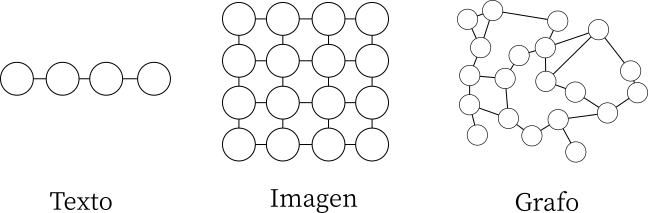
\includegraphics[width=0.8\linewidth]{img/img_texto_imagen_grafo.png}
  \caption{Los casos de procesamiento de texto y de imágenes se pueden pensar como instancias particulares del problema de grafos.}
  \label{fig:boat1}
\end{figure}


Sobre los tipos de modelos de redes neuronales sobre grafos, podemos dividir el
análisis en los siguientes grupos: 

\begin{itemize}  
\item Las redes convolucionales de grafos, tanto las que trabajan sobre el espacio
de frecuencia a través del laplaciano como las que trabajan en el espacio de tiempo
a través de otros métodos.
\item Las redes de grafos con modelos de atención.
\item Las basadas en otros métodos, como el movimiento de la red a lo largo del grafo.
\end{itemize}

Por completitud y para proveer un \textit{baseline}, también describiremos dos maneras
de utilizar métodos tradicionales de aprendizaje automático teniendo en cuenta la estructura
del grafo: utilizando términos de regularización y los que utilizan \textit{embeddings}.

En el caso general, el objetivo de las redes de grafos es aprender una función que toma
como entrada una señal sobre el grafo y la matriz de adyacencia\cite{kipf2016gcn}. 
Cada capa puede usar ambas entradas para armar mejores representaciones, 
como por ejemplo:
\begin{equation*}
    \Large
    h^{l+1} = f(h^l, A) = \bar\sigma A h^l W^l
\end{equation*}

Esta función genera una propagación de la señal $h^l$ transformada por $W^l$ a
los vecinos de cada nodo. Sin embargo, como $A_{ii} = 0 \forall i$, no tenemos
en cuenta la señal del propio nodo en su representación de $h^l$ para calcular
la de $h^{l+1}$. Esto se puede resolver usando $A+I$, u otros métodos que describiremos
luego.

En la mayoría de los casos vamos a usar capas ocultas $h^i$ con una dimensión constante
para los nodos, de manera que cada nodo tiene una representación que va cambiando a lo
largo de toda la red. Si el problema es de predicción a nivel nodo se mantiene hasta la
capa final, si el objetivo es predecir una propiedad del grafo entonces se puede poner un
\textit{softmax} como última capa. 

En \cite{zhou2018graphreview} se observa que para obtener un \textit{embedding} de cada
nodo utilizando una función que propague la información a lo largo de la red se puede
aplicar la misma función sucesivamente. Por el teorema del punto fijo de Banach, si
$f$ es una aplicación contractiva la convergencia de $x_n = f(x_{n-1})$ es exponencial.

% explicar las cosas en común a las topologías (punto fijo, etc.)

\subsubsection{Redes convolucionales de grafos}

%imagenet classification w/ dcn
En redes neuronales convolucionales de imágenes el operador fundamental es la convolución de
matrices. Esta operación es similar a la de un perceptrón multicapa, pero difiere en que 
se comparten los parámetros para todos los píxeles. La imagen se convoluciona con una
matriz \textit{kernel} para generar un \textit{feature map} que estará en la siguiente capa.
Esto permite encontrar filtros que detecten patrones sin importar dónde ocurran en la imagen.
Adicionalmente, aplicar varias capas convolucionales permite ir generando \textit{features}
de mayor orden; en la primera capa, cada píxel del \textit{feature map} corresponderá a un
vecindario de la imagen original, en la segunda, a un vecindario de vecindarios, etc. \cite{lecun1998gradient}
Las neuronas superiores tienen información global de la imagen.

En el caso de grafos estamos interesados en lo mismo, obtener información global del grafo en
representaciones superiores. Pero no es directa la generalización de la convolución -- 
en un grafo, el vecindario de un nodo es variable. No hay un \textit{orden} en los grafos
como lo había en imágenes. Para poder definir la convolución de una señal en un grafo se utiliza
la generalización discreta del laplaciano continuo.

El laplaciano combinatorio de un grafo se define como $L(G) = D-A$, donde $D$ es la matriz
de grados y $A$ la matriz de adyacencia. Si además definimos una señal sobre el grafo ---
a cada nodo le asignamos un valor según una función $f: V \rightarrow \mathbb{R}$ ---
podemos ver que $L(G)$ mapea $f$ a otra función $g$ de manera que $g = \nabla f$ \cite{whatsuplaplacian}.
Esto lo podemos %what's up with the graph laplacian
verificar si representamos a $f$ y $g$ como vectores columna, donde $f(i)$ es la iésima fila,%Wh
que es el valor del nodo $i$. Entonces: 

\begin{equation*}
\Large
g(i) = \sum_{j:(i,j) \in E} f(i)-f(j)    
\end{equation*}


esta operación define un orden sobre el grafo: el gradiente de una señal es,
para cada nodo, la sumatoria entre las diferencias entre su valor y el valor de
su vecino. Como es invariante respecto al índice, la operación entre dos grafos
isomorfos da el mismo resultado \cite{atwood2016dcnn}.
De la misma manera que en el caso continuo las autofunciones del operador
de Laplace forman la base para la transformada de Fourier, se puede hallar la transformada
de Fourier del grafo utilizando los autovectores de $L(G)$ \cite{graphfourier}. 

Esta analogía permite reutilizar el resultado clásico de señales continuas: 
$\mathcal{F}\{f*g\} = \mathcal{F}\{f}}\cdot \mathcal{F}\{g\}$ (la transformada de la convolución es la
multiplicación de las transformadas). Para poder hacer
convoluciones en grafos simplemente podemos hacerlo en el dominio de la
frecuencia, a través del laplaciano \footnote{Para sencillez de notación, usaremos
$L = L(G)$ mientras no sea ambigüo.} $L$. Entonces una capa convolucional
en un grafo es (\cite{kipf2016gcn}): 

$$f(H_l, A) = \bar \sigma (L H_l W_l)$$


En DCNN \cite{atwood2016dcnn} se utiliza una convolución que también incluye
la información de los vecinos que están a más de un paso, y cada nodo
tiene una representación segun la cantidad de \textit{saltos} que se consideran.
Es decir, $\mathbf h$ no es de $|V| \times F$ sino que es un tensor de $|V|\times H \times F$,
donde $H$ es \textit{hops}. Las activación de un nodo para cada $k\in \{0..H-1\}$  se
calcula utilizando $P^k$, donde $P = D^{-1}A$. $P^k$ representa la probabilidad de
transición a cada nodo de una caminata aleatoria (\textit{random walk}) de $k$ pasos.

\subsubsection{Redes con mecanismos de atención}

En procesamiento de lenguaje natural los mecanismos de atención han sido fundamentales
para mejor utilizar la información codificada en un vector. En \cite{attentionalyouneed}
se reemplazan las convoluciones y recurrencias normalmente utilizadas en modelos
de transducción por operaciones de atención. Una operación de atención es una función
que para cierta consulta asigna un peso a valores distintos. Por ejemplo, en un caso
de traducción para traducir el verbo no es necesario usar toda la oración; es posible
ignorar algunas palabras y enfatizar otras.

La atención es particularmente útil en casos de datos de tamaño variable, por lo que
es natural su aplicación en grafos. En \cite{GAT} se define un coeficiente de atención entre
dos nodos vecinos $i$ y $j$:

\begin{equation*}
    \Large
    \alpha_{ij} = \mathrm{softmax}_j(a(Wh_i, Wh_j))
\end{equation*}

donde $h_i$ y $h_j$ son las representaciones de los nodos $i$ y $j$ respectivamente,
$W$ es una matriz que transforma inicialmente las representaciones y $a$ es una función (por ejemplo,
una capa de funciones de activaciones LeakyReLU). $\alpha_{ij}$ sólo se
calcula entre vecinos, y la capa softmax se encarga de normalizar los valores.

Cuando se utiliza el laplaciano, los filtros que se aprenden dependen directamente
de los autovectores de la matriz\footnote{A diferencia de trabajar con señales en $\mathbb{R}$, 
la base de Fourier puede cambiar según el grafo que se utilice.}. Si los grafos que
se tienen poseen estructuras
distintas no es posible la generalización \cite{monti2017geometric} \cite{GAT}. 
La atención se puede ver como un mecanismo
local en el dominio del tiempo que puede manejar vecindarios de tamaños distintos, con
el beneficio de ser altamente paralelizable.


\subsubsection{Modelos tradicionales adaptados a grafos}

Una alternativa a usar modelos que por construcción incorporan propiedades del
grafo es intentar darle a modelos tradicionales información que represente
la estructura del grafo. 

\textbf{node2vec} \cite{grover2016node2vec} es un algoritmo que aprende \textit{embeddings}
en base a caminos aleatorios del grafo. Se diseña una política markoviana de segundo orden
para explorar el grafo, con hiperparámetros que balancean explorar el grafo o quedarse en
vecindarios locales. Cada camino aleatorio se puede pensar como una oración que luego se
pasa a un modelo Skip-gram. Los embeddings aprendidos por este modelo se pueden agregar
como \textit{features}; de esta manera, un modelo predictivo que trabaje sólo con datos
en formato de tabla puede aprovechar información de la estructura del grafo.

Otra opción es utilizar términos de regularización para hacer que la función de predicción
sea \textit{suave} sobre el grafo\cite{seeingstars_regularization}. Principalmente, la idea
es que dos nodos $i,j$ con arista de peso $w_{ij}$ deberían ser predichos de manera similar.
Basta agregar a la función objetivo $\mathcal{L}$ un término como $w_{ij} (f(x_i)-f(x_j))^2$,
donde $f$ es la predicción. Este método es agnóstico al modelo: mientras soporte nuevos términos
en la función de costo, se puede aplicar. También es posible extender esta idea a problemas
semi-supervisados, donde sólo se tiene una fracción de los nodos etiquetados.

\subsection{Predicción de sitios de unión}

En su descripción fundamental, la predicción de sitios de unión de una proteína
nueva se realiza en base a múltiples sitios de unión de proteínas y ligandos
anteriormente vistos. Una manera de hacerlo es, dada una consulta, buscar
proteínas similares y hacer una predicción en base a esos sitios de unión. En 
\cite{yang2013tmsite} se desarrolla un método de este tipo. Se desarrollan dos
componentes, \texttt{TM-SITE} y \texttt{S-SITE}, que utilizan las estructuras
y secuencias respectivamente.

\texttt{TM-SITE} intenta balancear una comparación global que alinea las estructuras
de dos proteínas -- que es robusta pero puede no alinear sitios locales de unión (LBS)
por una diferencia estructural en otra parte de la proteína -- con una comparación de subestructuras,
que es más sensible a similitudes locales pero puede tener un gran nivel de falsos positivos. 
Para esto, como pre-procesamiento, para todos los \textit{templates} (proteínas ya conocidas
en la base de datos) se calculan sus cavidades y se seleccionan todas las que tengan
átomos pesados en ellas como sitios posibles de unión. Dada una consulta específica, se
hace un alineamiento contra los \textit{templates} y se calcula un puntaje para cada uno. A
modo ilustrativo, la ecuación del puntaje es:

\begin{equation*}
    \LARGE 
    q_{str} = \frac{2}{1+\exp\{-[L_c(0.4L_g+0.3L_s+0.2JSD)+TM]^2\}} - 1
\end{equation*}

que utiliza el porcentaje de los aminoácidos alineados a la consulta ($L_c$),
la similitud estructural entre las cavidades ($L_g$), la relación evolutiva entre
los pares alineados ($L_s$, según puntaje \texttt{BLOSUM62}), el índice de conservación
de la secuencia y un puntaje del alineamiento (TM). Una vez obtenidos los candidatos
con $q_{str} > 0.65$, se superponen los ligandos en la consulta y se agrupan en
\textit{clusters} según sus centros geométricos. Cada grupo luego vota sobre los
aminoácidos de la cavidad que participan en la unión, y se decide por mayoría.

Por otro lado, \texttt{S-SITE} trabaja a nivel secuencia. Se transforma la consulta
a una matriz de frecuencias y se busca un \textit{match} contra las matrices pre-calculadas
en la base de datos. Se utiliza una ecuación de puntaje similar en forma a la anterior,
pero en vez de información estructural se usa la información de alineamientos de secuencia.
También se aumenta el puntaje si en el alineamiento de secuencias los residuos coinciden
en el rol de la estructura secundaria (predicha por otro programa, \texttt{STRIDE}). Similar
a \texttt{TM-SITE}, se arma un consenso para elegir cuáles de los residuos participan
en la unión.

Finalmente, \texttt{COACH} es una SVM a la cual se le pasan los resultados de \texttt{S-SITE},
\texttt{TM-SITE}, \texttt{COFACTOR}, \texttt{FINDSITE} y \texttt{ConCavity}.

En \textbf{ATPbind}\cite{atpbind} se utiliza un acercamiento similar pero con únicamente el objetivo de
predecir uniones con ATP. La razón para condicionar a un solo ligando es que se puede
obtener una precisión superior: aproximar la distribución conjunta de probabilidad de unión
requiere modelar (explícita o implícitamente) los distintos tipos de interacciones, mientras
que aproximar la probabilidad de unión condicionada a un ligando en particular no.

A nivel metodológico, se usan versiones modificadas de
\texttt{TM-SITE} y \texttt{S-SITE}. Por el imbalance de clases (aproximadamente 25 a 1)
se utliza \textit{random undersampling} y se arma un \textit{mean ensemble scheme} con
10 SVMs. Si bien el resultado es bueno (AUC $93.5\%$), el gran tamaño del modelo hace
que predecir cada instancia sea muy lento\footnote{En \cite{atpbind} se menciona
que para una proteína de 300 aminoácidos el modelo predice sus sitios de unión
en un poco menos de una hora.}.

Otra manera de representar a las proteínas es no por su estructura (sea primaria,
secundaria o terciaria), sino por cómo se comporta ante distintos ligandos. Es decir,
se pueden comparar las proteínas en base a la similaridad de los ligandos que se
unen a ellos \cite{keiser2009newtargetsknowndrugs} \cite{keiserhert2008relatingdrugclasses}.
Agrupando ligandos según la similaridad de sus \textit{fingerprints}\footnote{Un \textit{fingerprint}
es un vector con bits que se prenden según la presencia de algún grupo funcional, formato o
propiedad en la droga.}, se arman 
clases que se utilizan para representar proteínas. Se puede entonces predecir
nuevas interacciones para proteínas y drogas conocidas, con el punto clave de que
las proteínas no necesariamente están relacionadas evolutivamente o por sus
estructuras.

En \cite{fout2017proteininterface} se aplican redes convolucionales de grafos para
predecir interfases entre proteínas. Puntualmente, hacen predicciones centradas en
cada nodo:
\begin{equation*}
    \LARGE
    z_i = \sigma\left ( W_C x_i + \frac{1}{\mathcal{N}_i} \sum_{j\in \mathcal{N}_i} W_N x_j + b \right )
\end{equation*}

donde $W^C$ es una matriz de pesos para el nodo central (pero compartida entre cada
predicción), $W^N$  una matriz de pesos para los nodos vecinos, 
$x_i$ y $x_j$ son \textit{features} de los nodos $i$ y $j$, $\mathcal{N}_i$ es el conjunto
de vecinos de $i$. Un punto clave de \cite{fout2017proteininterface} es que no pueden
usar el laplaciano porque las proteínas del conjunto de datos no tienen correspondencia
natural. Dado ese caso, utilizan convoluciones espaciales y no en el dominio de frecuencia.




% adverse side effects
% describir estructura secundaria
% leer sobre PSFM, PSSM
%COFACTOR?
%problema de similaridad => CDHit
%otro metodo es. .. . predecir!
%pocket detection
%sequence alignment como feature => explicar

%fingerprinting de moleculas si uno quiere laburar con varios ligandos => paper colwell


%node2vec, regularización en xgboost, difusión de propiedades
%graph attention networks <- Protein-Protein Interaction dataset
%paper de comparación (review) 


\subsection{Consideraciones especiales} \label{consideraciones}

Se ha sugerido\cite{wallach2018overfitting} que muchos modelos predictivos de
uniones de ligandos tienen \textit{overfitting}. Esto se debe a que, a diferencia
de otros dominios, en este problema no es suficiente hacer una
partición de datos en entrenamiento, validación y test. Existen redundancias
de proteínas (dos proteínas con códigos distintos que son la misma), o similitudes
evolutivas (la hemoglobina del humano es muy parecida a la hemoglobina del caballo) que
si no se tienen en cuenta hacen de una división aleatoria una mala opción.

Por ejemplo, para \textbf{ATPbind} \cite{atpbind} se descartan las secuencias con
similitud mayor a 40\%. Para tener analizar las similitudes y relaciones evolutivas,
se pueden utilizar bases de datos como CDHit\footnote{\url{http://www.bioinformatics.org/cd-hit/}} o
Pfam\footnote{\url{http://pfam.xfam.org/}}.

%Papers de meta-análisisaplicaciones laplaciano no funciona siempre overfitting algo de pfam, cdhit

\newpage
\section{Propuesta y objetivos}
% Explicar idea general. 
% Contribuciones
En este trabajo interpretamos que el problema de unión con una proteína no depende 
de las posiciones absolutas de sus aminoácidos, sino que es un problema de la
\textit{conectividad} que tienen en el espacio. Dado esto, es natural usar una
estructura de grafo para codificar el problema. Las redes neuronales de grafos
utilizan entonces propiedades topológicas: un nodo no recibirá información
de otro nodo en capas siguientes si no están en la misma componente conexa. De
la misma manera, hay más pasaje de información entre comunidades y en regiones
densas de conexiones. Además, el uso
de un grafo tiene varios beneficios, ya que es invariante a rotaciones y 
traslaciones en el espacio e inmediatamente codifica cuándo hay una unión y cuándo
no. De otra manera, un modelo predictivo que parte desde las ubicaciones físicas 
de los átomos debe además modelar y representar estas invariantes, lo que complejiza
aún más el problema.

%mencionar que se hace en el instituto de cálculo y en FIUBA
Esta noción no es nueva. En \cite{fout2017proteininterface} se utiliza un grafo
donde los nodos son los aminoácidos de la proteína y hay arista si están hasta
cierta distancia (e.g. 4\r{A}). En esta tesis proponemos usar otro método, 
que es a través de técnicas de homología persistente \cite{edelsbrunner2008perseus}. 
Esencialmente, la idea es construir un complejo simplicial de manera
iterativa hasta capturar las propiedades topológicas fundamentales de la estructura.
A partir de esto se puede construir un grafo que codifique las cavidades, agujeros, y
otras propiedades\footnote{La construcción de este grafo ya está hecha y es la base
de esta tesis, gracias al trabajo de Leonardo Córdoba y Leandro Lombardi (2019).}.


El componente novedoso de este trabajo es utilizar redes neuronales de grafos (GNNs) sobre
las estructuras para poder predecir la unión entre ligandos y drogas. Se han utilizado
GNNs para predecir interfases entre proteinas \cite{fout2017proteininterface}, y se han 
utilizado GNNs para representar drogas \cite{tsubaki2018CPIgnn}, pero no para el problema 
de representar a la proteína y en \textit{binding site prediction}. 

En principio, el objeto de estudio es investigar cómo funciona este tipo de redes
sobre uniones entre proteínas y ATP, tal como se hace en \textbf{ATPbind}\cite{atpbind}.
Como se ha mencionado, al condicionar en un solo tipo de ligando el problema se
simplifica porque no es necesario explorar o modelar todo el espacio de configuraciones 
físico-químicas.
Sin embargo, también se reduce mucho la cantidad de datos disponibles. Por ejemplo,
en la base de datos de PDB en principio solo hay 1369 estructuras con información de 
unión con el ATP -- este número será más pequeño cuando se filtren por cadenas
repetidas y similares.

Dado eso, proponemos investigar también cómo poder incorporar información adicional
para poder predecir uniones con ATP. La intuición detrás de esto es que tomar información
de cómo se comportan otros tipos de uniones (entre proteínas y otros ligandos) puede darle
mayor capacidad predictiva al modelo. Inicialmente, dos formas de lograr esto son posibles:   

\begin{itemize}
    \item \textbf{Incoporando información del ligando en el modelo}. Es la idea utilizada en
    \cite{tsubaki2018CPIgnn} y \cite{yang2013tmsite}. En principio, la idea es que se puede
    predecir más específicamente el comportamiento de los aminoácidos de la proteína
    contra el ligando. Esto agrega más modelado a la red pero puede facilitar la tarea de
    predicción. Otra forma de representar a la droga es
    con un \textit{embedding} en base a sus interacciones (idea similar a 
    \cite{keiser2009newtargetsknowndrugs}).
    \item \textbf{A través de \textit{transfer learning}}. Se puede plantear entrenar
    al modelo con otros tipos de interacciones para luego re-entrenar sólo con ATP.
    En este esquema se mantiene la forma del modelo -- prediciendo la unión de las proteínas con solo un ligando en particular -- pero en vez de entrenar la red desde un punto aleatorio se 
    parte desde un predictor genérico de sitios de unión. Esto es importante porque
    podemos utilizar muchos más datos del \textit{Protein Data Bank}. 
\end{itemize}

Finalmente, un punto interesante para analizar es el comportamiento del modelo. Son conocidos
varios análisis de interpretabilidad sobre redes convolucionales de 
imágenes\cite{olah2018interpretability}, y sobre
modelos de atención en texto\cite{attentionalyouneed}. Queremos, una vez entrenados
y probados los modelos,
poder visualizar qué rol tienen los pesos de atención y los \textit{feature maps} (en el caso
de convoluciones) para las redes neuronales de grafos. Idealmente, los patrones aprendidos
tienen relaciones o funciones biológicas. En línea con esta idea,
se pueden pensar esquemas de entrenamiento o arquitecturas que
se dispongan mejor al problema (por ejemplo, tal vez no es necesario entrenar con todo el grafo a la vez --- entrenar por subgrafos sería similar a predecir por regiones en imágenes).

Paralelamente, encontramos que no hay paquetes listos para usar que contemple la
transformación de estructuras en grafos para utilizarlos en modelos predictivos, ni
la creación o manipulación de \textit{folds} para validación cruzada que considere 
las particularidades anteriormente mencionadas (sección \ref{consideraciones}). Ya que
para este trabajo es necesario hacer ambos, disponibilizar este tipo de transformaciones
y algoritmos nos parece un aporte valorable para la comunidad científica.

En resumen, la propuesta tiene los siguientes objetivos:

\begin{enumerate}
    \item Probar redes neuronales basadas en grafos al problema de predicción 
    de sitio de unión entre proteínas y el ATP.
    \item Investigar cómo incorporar información adicional del
    problema global de sitios de unión al caso de ATP.
    \item Interpretar el comportamiento aprendido del modelo en base a su sensibilidad
    a los datos y clases.
    \item Investigar qué modificaciones a la arquitectura de la red o al
    esquema de entrenamiento logran mejor precisión en la predicción.
    \item Disponibilizar un paquete de creación y manipulación de grafos de proteínas,
    junto con una manera de crear particiones para validación sin sesgos
    biológicos-estadísticos.
\end{enumerate}

%decir qué ligandos => biolip, datos de PDB, estructuras que estan ahí o usando ITasser,
%métricas AUC pero ver el AVE
%baselines => cavity, node2vec + xgboost, coach + atpbind, 

\subsection{Experimentos}\label{experimentos}

Los datos a utilizar en los experimentos son tomados de PDB. Sin embargo, como no
todos los ligandos en la base de datos son importantes, usaremos
información curada en BioLiP\cite{yang2012biolip} que tiene interacciones de proteínas y ligandos
biológicamente relevantes.

Los experimentos a realizar son:

\begin{itemize}
    \item \textbf{Experimento 1.} Predecir uniones proteína-ATP con un conjunto de datos similar al de \textbf{ATPbind}
    \cite{atpbind} y redes neuronales convolucionales de grafos. En principio, no todas las proteínas usadas tienen estructuras, que 
    es requisito para nuestro modelo. Será necesario entonces predecir la estructura con
    un software o reducir el conjunto de datos a los que sólo tienen estructura. 
    \item \textbf{Experimento 2.} Repetir el experimento pero con redes neuronales
    de atención en grafos, y con otros mecanismos de convoluciones espaciales y
    espectrales.
    \item \textbf{Experimento 3.} Probar otros tipos de grafos, como un grafo de
    contactos \cite{fout2017proteininterface}. 
    \item \textbf{Experimento 4.} Incorporar información adicional al modelo en base
    a otras interacciones relevantes de las proteínas \cite{yang2012biolip} o a
    representaciones distintas \cite{keiser2009newtargetsknowndrugs}.
    \item \textbf{Experimento 5.} Hacer algunas modificaciones a las arquitecturas
    de las redes o a la forma de entrenamiento para que el modelo se ajuste más
    al dominio del problema.
\end{itemize}

Como métricas usaremos principalmente el área bajo la curva ROC (AUC), pero atendiendo
a las métricas de overfitting enunciadas en \cite{wallach2018overfitting}.

Aparte del grafo, usaremos \textit{features} adicionales como accesibilidad de un nodo
a la superficie, qué tipo de aminoácido es, su carga e hidrofobicidad, descriptores de la
forma, accesibilidad de solventes y otros valores estándares en la literatura.

En todos los casos usaremos como \textit{baseline} una detección de cavidades, que simplemente
encuentra agujeros donde habría potencialmente un sitio de unión (mismo que en \cite{yang2013tmsite}). Como comparación usaremos \texttt{TM-SITE}, \textbf{ATPbind}
y otros modelos anteriormente citados.

Finalmente, experimentaremos maneras de darle interpretación al modelo. Esto puede
ser visualizar el laplaciano y su variación a lo largo de proteínas y estructuras 
distintas,
ver qué nodos son más ponderados en los mecanismos de atención, y observar la localidad
de la predicción, entre otros posibles análisis.

%otra dimensión de prueba es parchecitos y lidiar con unme

\newpage
\section{Cronograma de trabajo}

A continuación se detalla una estimación de la cantidad de horas que llevará cada tarea,
y la relación entre ellas. 

\begin{table}[h]
\begin{tabular}{|l|l|l|l|l|l|l|l|l|l|l|l|l|}
\hline
\multicolumn{1}{|c|}{}                         & \multicolumn{12}{c|}{Meses}                                                                                                                                                                                                                                                                                                                                                                                                                                                 \\ \cline{2-13} 
\multicolumn{1}{|c|}{\multirow{-2}{*}{Tareas}} & 1                                               & 2                                               & 3                        & 4                        & 5                                               & 6                        & 7                                               & 8                                               & 9                        & 10                                              & 11                       & 12                       \\ \hline
Análisis de literatura                         & \cellcolor[HTML]{000000}{\color[HTML]{000000} } & \cellcolor[HTML]{000000}{\color[HTML]{000000} } &                          &                          &                                                 &                          &                                                 &                                                 &                          &                                                 &                          &                          \\ \hline
Desarrollo de pipeline                         &                                                 & \cellcolor[HTML]{000000}                        & \cellcolor[HTML]{000000} &                          &                                                 &                          &                                                 &                                                 &                          &                                                 &                          &                          \\ \hline
Construcción de modelos                        &                                                 &                                                 & \cellcolor[HTML]{000000} & \cellcolor[HTML]{000000} & \cellcolor[HTML]{000000}{\color[HTML]{000000} } &                          &                                                 &                                                 &                          &                                                 &                          &                          \\ \hline
Experimentación                                &                                                 &                                                 &                          &                          & \cellcolor[HTML]{000000}                        & \cellcolor[HTML]{000000} & \cellcolor[HTML]{000000}                        & \cellcolor[HTML]{000000}                        & \cellcolor[HTML]{000000} &                                                 &                          &                          \\ \hline
Comparación y revisión                         &                                                 &                                                 &                          &                          &                                                 &                          & \cellcolor[HTML]{FFFFFF}{\color[HTML]{000000} } & \cellcolor[HTML]{000000}{\color[HTML]{000000} } & \cellcolor[HTML]{000000} &                                                 &                          &                          \\ \hline
Análisis e Interpretación                      &                                                 &                                                 &                          &                          &                                                 &                          &                                                 &                                                 & \cellcolor[HTML]{000000} & \cellcolor[HTML]{000000}{\color[HTML]{000000} } &                          &                          \\ \hline
Redacción de tesis                             &                                                 &                                                 &                          &                          &                                                 &                          &                                                 &                                                 &                          & \cellcolor[HTML]{000000}{\color[HTML]{000000} } & \cellcolor[HTML]{000000} & \cellcolor[HTML]{000000} \\ \hline
\end{tabular}
\end{table}

Para las estimaciones se toma como base una ocupación de doce horas semanales. La carga total es de 648 horas.

\begin{itemize}
 \renewcommand{\labelitemi}{\scriptsize$\blacksquare$}
 \item  \textbf{Análisis de literatura} [81 horas]. Esta tarea es la de familiarización con la literatura, con
 modelos actuales del problema y las posibilidades de innovación.
 \item  \textbf{Desarrollo de pipeline} [54 horas]. El \textit{pipeline} son todos los
 pasos para una corrida completa, desde tomar las proteínas de la base de datos PDB,
 procesarlas para conseguir los grafos y sus \textit{features} hasta terminar con
 un modelo entrenado en \textit{folds} sin sesgos estadístico-biológicos.
 \item  \textbf{Construcción de modelos} [108 horas].   Los modelos de redes
 neuronales de convolución de grafos y de atención se deben construir en base a la
 literatura preexistente y deben ser ajustados para el problema en cuestión. En 
 esta parte además se pueden analizar qué componentes de las redes pueden ser variados
 para luego encontrar una mejor solución al problema.
 \item  \textbf{Experimentación} [180 horas]. En esta fase se llevan a cabo
 todos los experimentos enunciados en la propuesta.
 \item  \textbf{Comparación y revisión} [45 horas]. Se revisan los resultados del modelo,
 se lo compara con los trabajos anteriormente citados y se hacen controles sobre
 los experimentos.
 \item  \textbf{Análisis e Interpretación} [45 horas]. En esta parte nos interesa
 entender cómo funcionan los modelos implementados, desde un análisis de sensibilidad
 hasta un entendimiento de los filtros aprendidos.
 \item  \textbf{Redacción de tesis} [135 horas]. En la tesis final estarán compiladas
 todas las fases anteriores, por lo que aparte de la redacción también implica revisar
 los pasos previos.
\end{itemize}



%--------------------------------------------
% Literatura
%--------------------------------------------
\newpage
\printbibliography

%--------------------------------------------
% Spisy (opcjonalne)
%--------------------------------------------
\newpage

% Wykaz symboli i skrótów.
% Pamiętaj, żeby posortować symbole alfabetycznie
% we własnym zakresie. Ponieważ mało kto używa takiego wykazu, 
% uznałem, że robienie automatycznie sortowanej listy
% na poziomie LaTeXa to za duży overkill. 
% //AB
%\vspace{0.8cm}
%\begin{acronym}
    %\item \textbf{EiTI} -- Facultad de Ingenieria
    %\item \textbf{PW} -- Universidad de Buenos Aires
%\end{acronym}
\vspace{1cm}                % vertical space

%\listoffigures              % Spis obrazków. 
%\vspace{1cm}                % vertical space
%\listoftables               % Spis tabel. 
%\vspace{1cm}                % vertical space
%\begin{appendix}            % Spis załączników.  
    %\item Załącznik 1.
    %\item Załącznik 2.
%\end{appendix}

% Możesz też dodać swój własny spis, 
% np. spis algorytmów. 
% \begin{spis}{algorytmów}
%     \item Algorytm 1.
%     \item Algorytm 2.
% \end{spis}

\end{document} % Dobranoc. 

